%----------------------------------------------------------------------------------------
%   Доорх хэсгийг өөрчлөх шаардлагагүй
%----------------------------------------------------------------------------------------
%!TEX TS-program = xelatex
%!TEX encoding = UTF-8 Unicode
\documentclass[12pt,A4]{report}

\usepackage{fontspec,xltxtra,xunicode}
\setmainfont[Ligatures=TeX]{Times New Roman}
\setsansfont{Arial}

% \usepackage[utf8x]{inputenc}
% \usepackage[mongolian]{babel}
%\usepackage{natbib}
\usepackage{geometry}
%\usepackage{fancyheadings} fancyheadings is obsolete: replaced by fancyhdr. JL
\usepackage{fancyhdr}
\usepackage{float}
\usepackage{afterpage}
\usepackage{graphicx}
\usepackage{amsmath,amssymb,amsbsy}
\usepackage{dcolumn,array}
\usepackage{tocloft}
\usepackage{dics}
\usepackage{nomencl}
\usepackage{upgreek}
\newcommand{\argmin}{\arg\!\min}
\usepackage{mathtools}
\usepackage[hidelinks]{hyperref}

\usepackage{algorithm}
\usepackage{algpseudocode}
\usepackage{color}
\definecolor{codegreen}{rgb}{0,0.6,0}
\definecolor{codegray}{rgb}{0.5,0.5,0.5}
\definecolor{codepurple}{rgb}{0.58,0,0.82}
\definecolor{backcolour}{rgb}{0.99,0.99,0.99}
\definecolor{lightgray}{rgb}{.9,.9,.9}
\definecolor{darkgray}{rgb}{.4,.4,.4}
\definecolor{purple}{rgb}{0.65, 0.12, 0.82}

\usepackage{listings}
\DeclarePairedDelimiter\abs{\lvert}{\rvert}%
\makeatletter
\usepackage{caption}
\captionsetup[table]{belowskip=0.5pt}
\usepackage{subfiles}

\usepackage{listings}
\renewcommand{\lstlistingname}{Код}
\renewcommand{\lstlistlistingname}{\lstlistingname ын жагсаалт}

\lstdefinelanguage{TypeScript}{
  keywords={abstract, any, as, boolean, break, case, catch, class, console,
    const, continue, debugger, declare, default, delete, do, else, enum, export,
    extends, false, finally, for, from, function, get, if, implements, import, in,
    infer, instanceof, interface, keyof, let, module, namespace, never, new, null,
    number, object, package, private, protected, public, readonly, require, return,
    set, static, string, super, switch, symbol, this, throw, true, try, type, typeof,
    undefined, unique, unknown, var, void, while, with, yield, async, await},
  keywordstyle=\color{blue}\bfseries,
  ndkeywords={class, export, boolean, throw, implements, import, this},
  ndkeywordstyle=\color{darkgray}\bfseries,
  identifierstyle=\color{black},
  sensitive=false,
  comment=[l]{//},
  morecomment=[s]{/*}{*/},
  commentstyle=\color{purple}\ttfamily,
  stringstyle=\color{red}\ttfamily,
  morestring=[b]',
  morestring=[b]"
}

\lstset{
   language=TypeScript,
   backgroundcolor=\color{lightgray},
   extendedchars=true,
   basicstyle=\footnotesize\ttfamily,
   showstringspaces=false,
   showspaces=false,
   numbers=left,
   numberstyle=\footnotesize,
   numbersep=9pt,
   tabsize=2,
   breaklines=true,
   showtabs=false,
   captionpos=b
}
\lstdefinestyle{mystyle}{
    basicstyle=\ttfamily\small,
    backgroundcolor=\color{backcolour},
    commentstyle=\color{codegreen},
    keywordstyle=\color{magenta},
    numberstyle=\tiny\color{codegray},
    stringstyle=\color{codepurple},
    %basicstyle=\footnotesize,
    breakatwhitespace=false,
    breaklines=true,
    captionpos=b,
    keepspaces=false,
    numbers=left,
    numbersep=10pt,
    showspaces=false,
    showstringspaces=true,
    showtabs=false,
    tabsize=2
}

\lstset{style=mystyle, label=DescriptiveLabel}

\let\oldabs\abs
\def\abs{\@ifstar{\oldabs}{\oldabs*}}
\makenomenclature
\begin{document}


%----------------------------------------------------------------------------------------
%   Өөрийн мэдээллээ оруулах хэсэг
%----------------------------------------------------------------------------------------

% Дипломийн ажлын сэдэв
\title{Блокчэйн суурьт лиценз баталгаажуулалт}
% Дипломын ажлын англи нэр
\titleEng{Licence validation with blockchain}
% Өөрийн овог нэрийг бүтнээр нь бичнэ
\author{Энхбаярын Жавхлан}
% Өөрийн овгийн эхний үсэг нэрээ бичнэ
\authorShort{Э.Жавхлан}
% Удирдагчийн зэрэг цол овгийн эхний үсэг нэр
\supervisor{Дэд  профессор Ч.Алтангэрэл}
% Хамтарсан удирдагчийн зэрэг цол овгийн эхний үсэг нэр
\cosupervisor{Д.Цолмон}
% СиСи дугаар
\sisiId{20B1NUM0649}
% Их сургуулийн нэр
\university{МОНГОЛ УЛСЫН ИХ СУРГУУЛЬ}
% Бүрэлдэхүүн сургуулийн нэр
\faculty{МЭДЭЭЛЛИЙН ТЕХНОЛОГИ, ЭЛЕКТРОНИКИЙН СУРГУУЛЬ}
% Тэнхимийн нэр
\department{МЭДЭЭЛЭЛ, КОМПЬЮТЕРИЙН УХААНЫ ТЭНХИМ}
% Зэргийн нэр
\degreeName{Бакалаврын судалгааны ажил}
% Суралцаж буй хөтөлбөрийн нэр
\programeName{Програм хангамж}
% Хэвлэгдсэн газар
\cityName{Улаанбаатар хот}
% Хэвлэгдсэн огноо
\gradyear{2024 он}


%----------------------------------------------------------------------------------------
%   Доорх хэсгийг өөрчлөх шаардлагагүй
%----------------------------------------------------------------------------------------
%----------------------Нүүр хуудастай хамаатай зүйлс----------------------------
\pagenumbering{roman}
\makefrontpage
\maketitle

\doublespace

% Decleration
\begin{huge}
\textbf{Зохиогчийн баталгаа}
\end{huge} \\ \ \\
\doublespace
Миний бие \@author \ "\@title" \ сэдэвтэй судалгааны ажлыг гүйцэтгэсэн болохыг зарлаж дараах зүйлсийг баталж байна:
\begin{itemize}
\item Ажил нь бүхэлдээ эсвэл ихэнхдээ Монгол Улсын Их Сургуулийн зэрэг горилохоор дэвшүүлсэн болно.
\item Бусдын хийсэн ажлаас хуулбарлаагүй, ашигласан бол ишлэл, зүүлт хийсэн.
\item Ажлыг би өөрөө (хамтарч) хийсэн ба миний хийсэн ажил, үзүүлсэн дэмжлэгийг тайлангийн ажилд тодорхой тусгасан.
\item Ажилд тусалсан бүх эх сурвалжид талархаж байна.
\end{itemize}
\

Гарын үсэг: \underline{\hspace{5cm}}

Огноо: 	\ \ \underline{\hspace{3cm}}

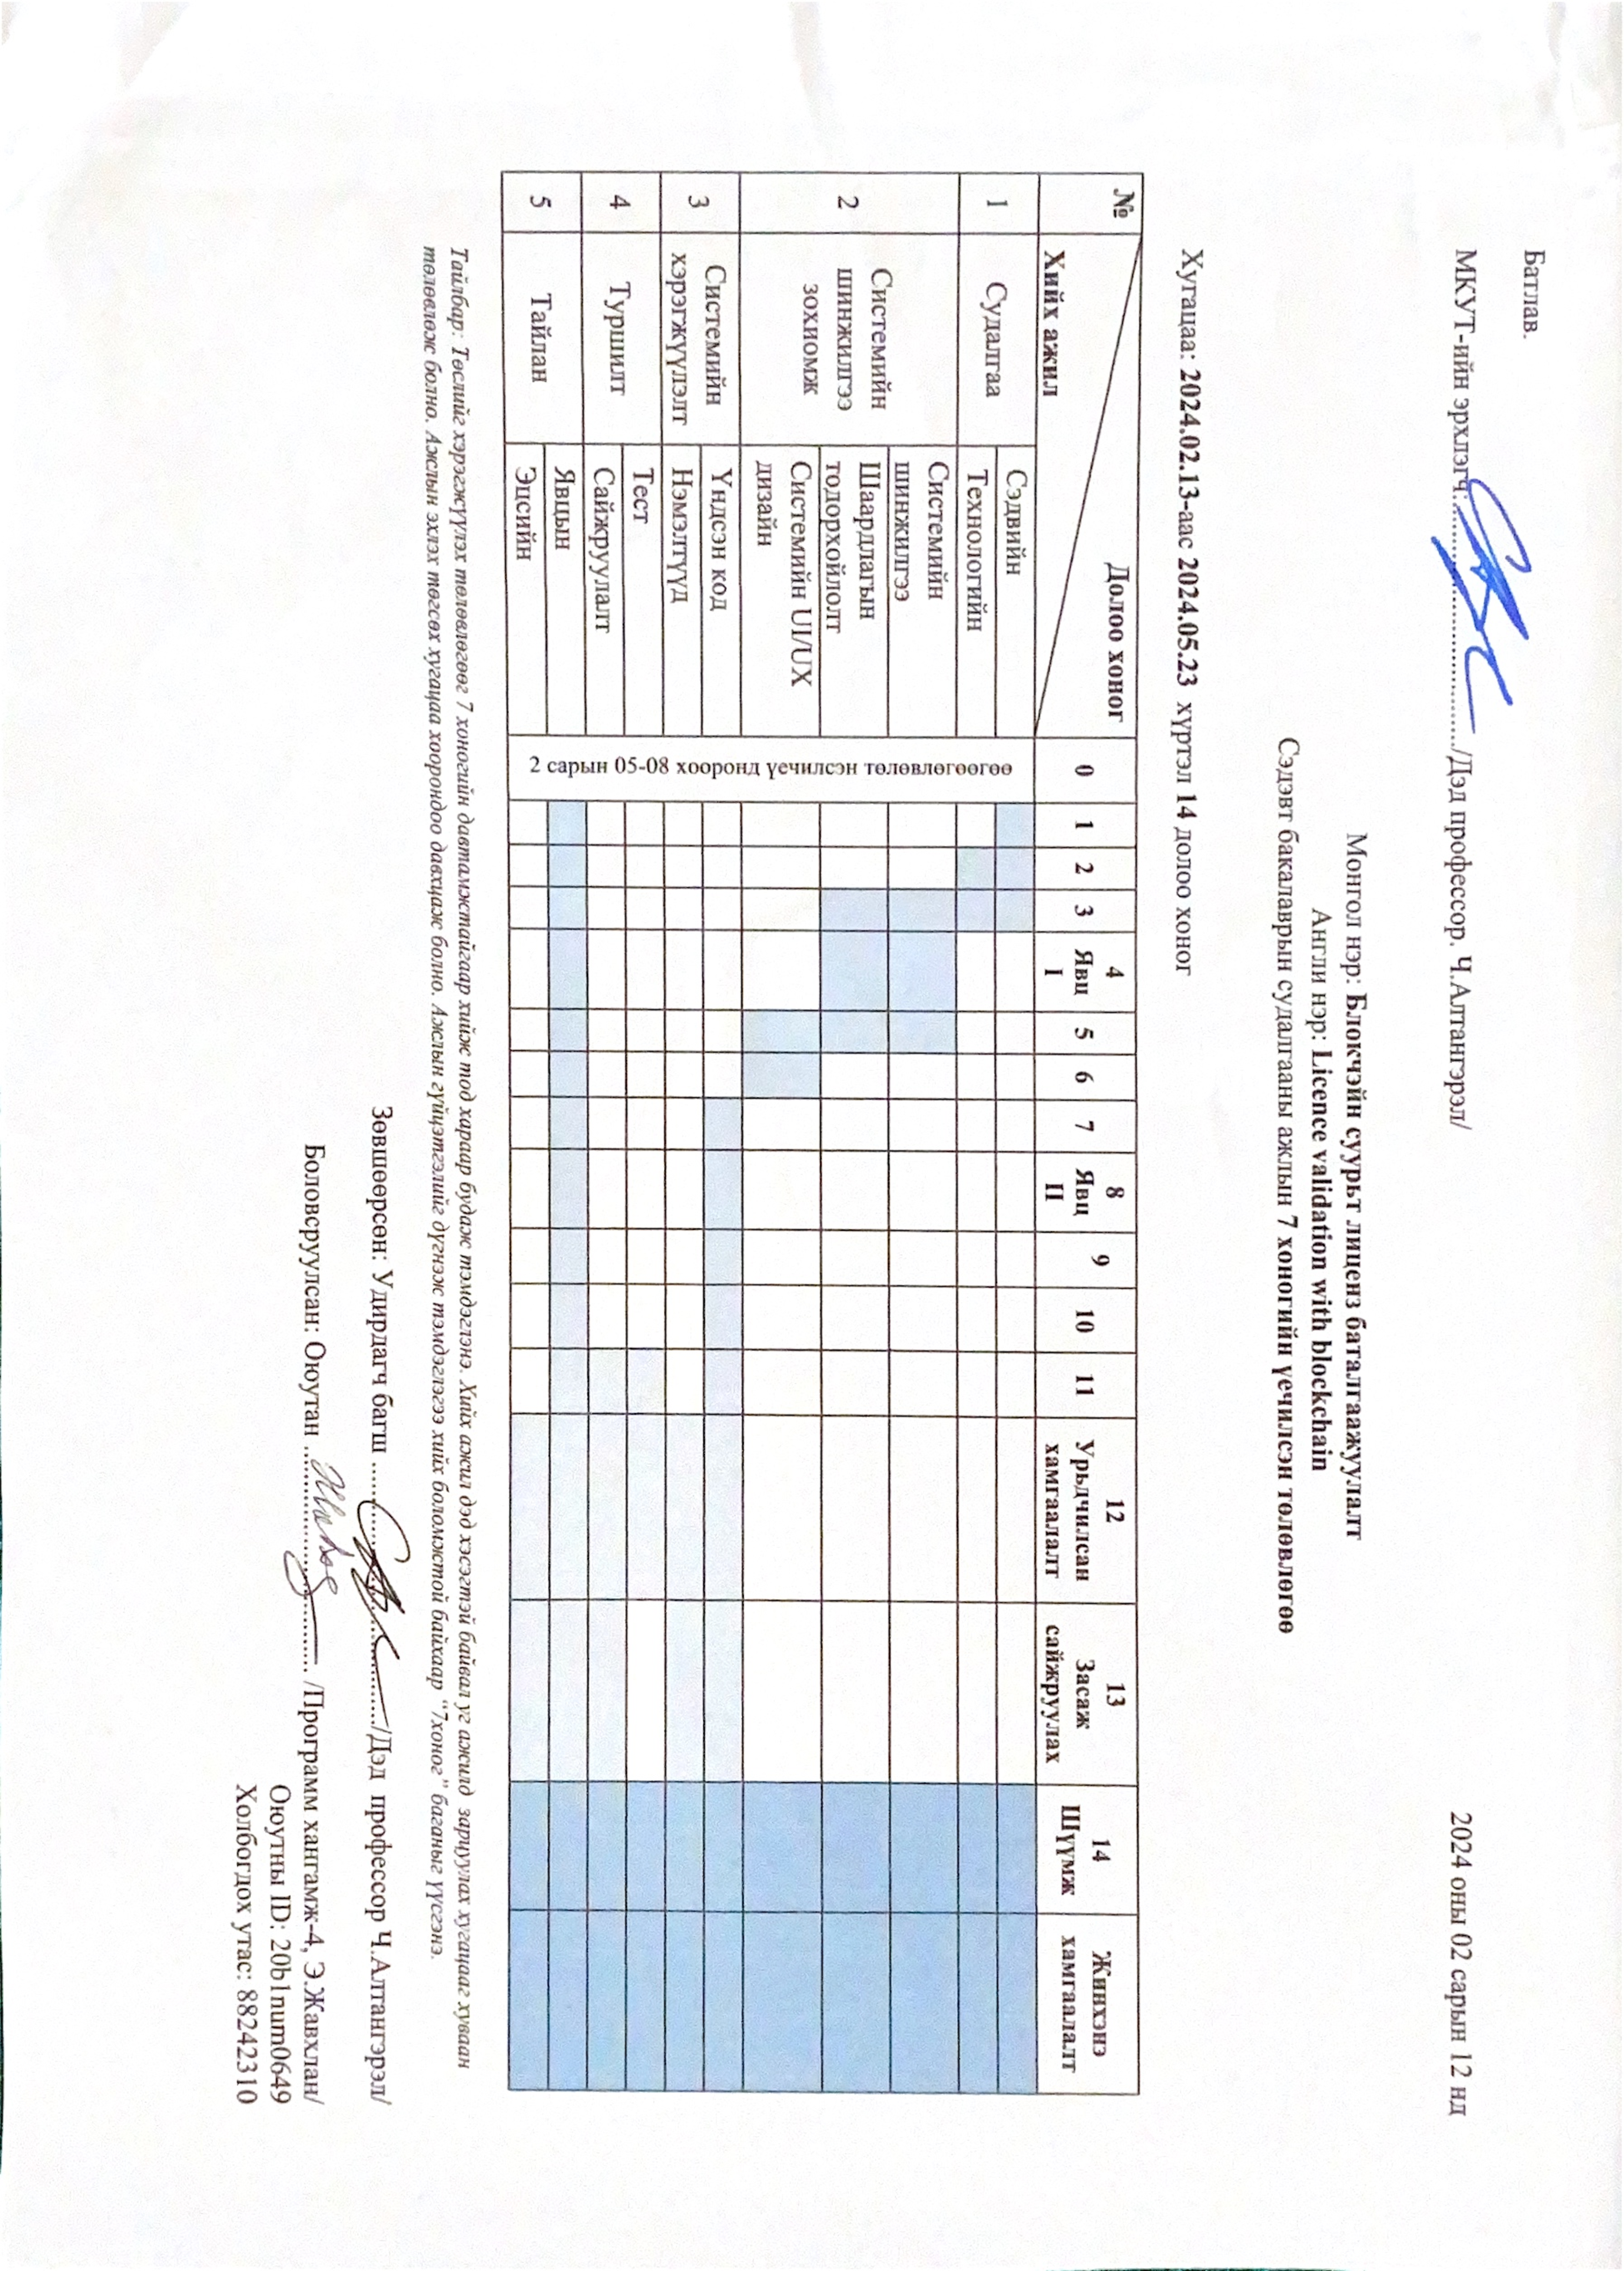
\includepdf[pages=1]{./src/periodic-table.pdf}
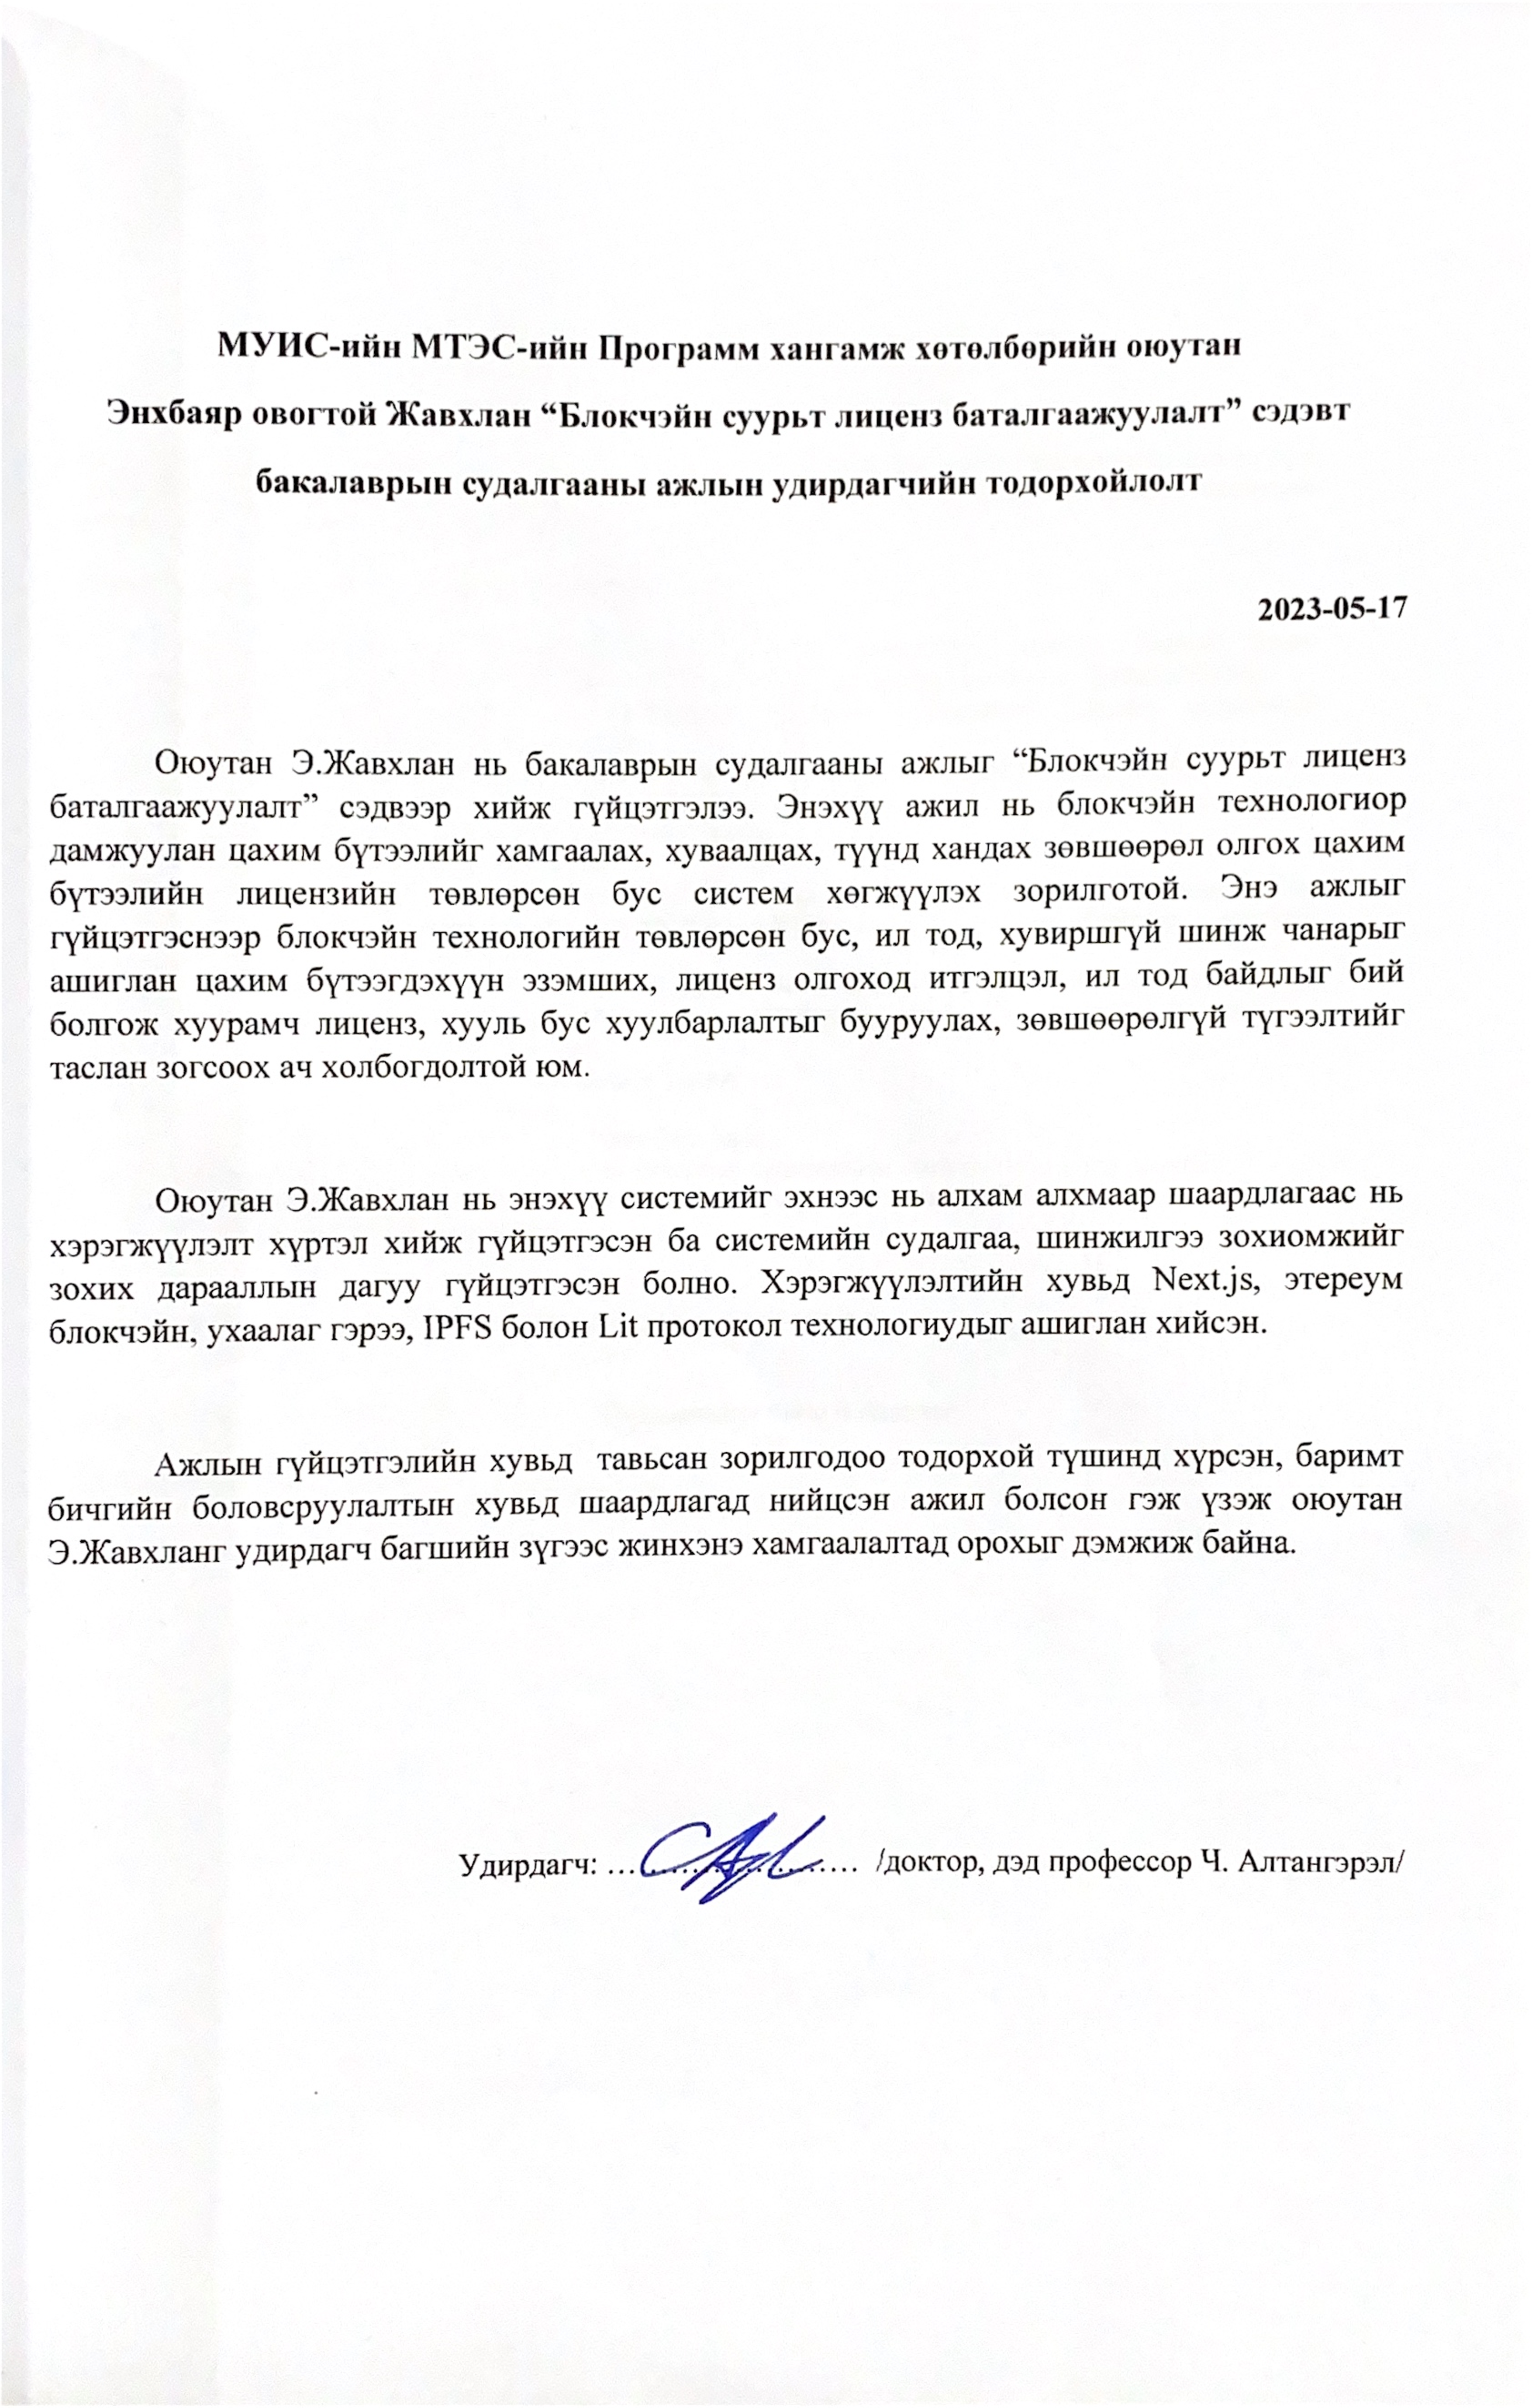
\includepdf[pages=1]{./src/todorh.pdf}
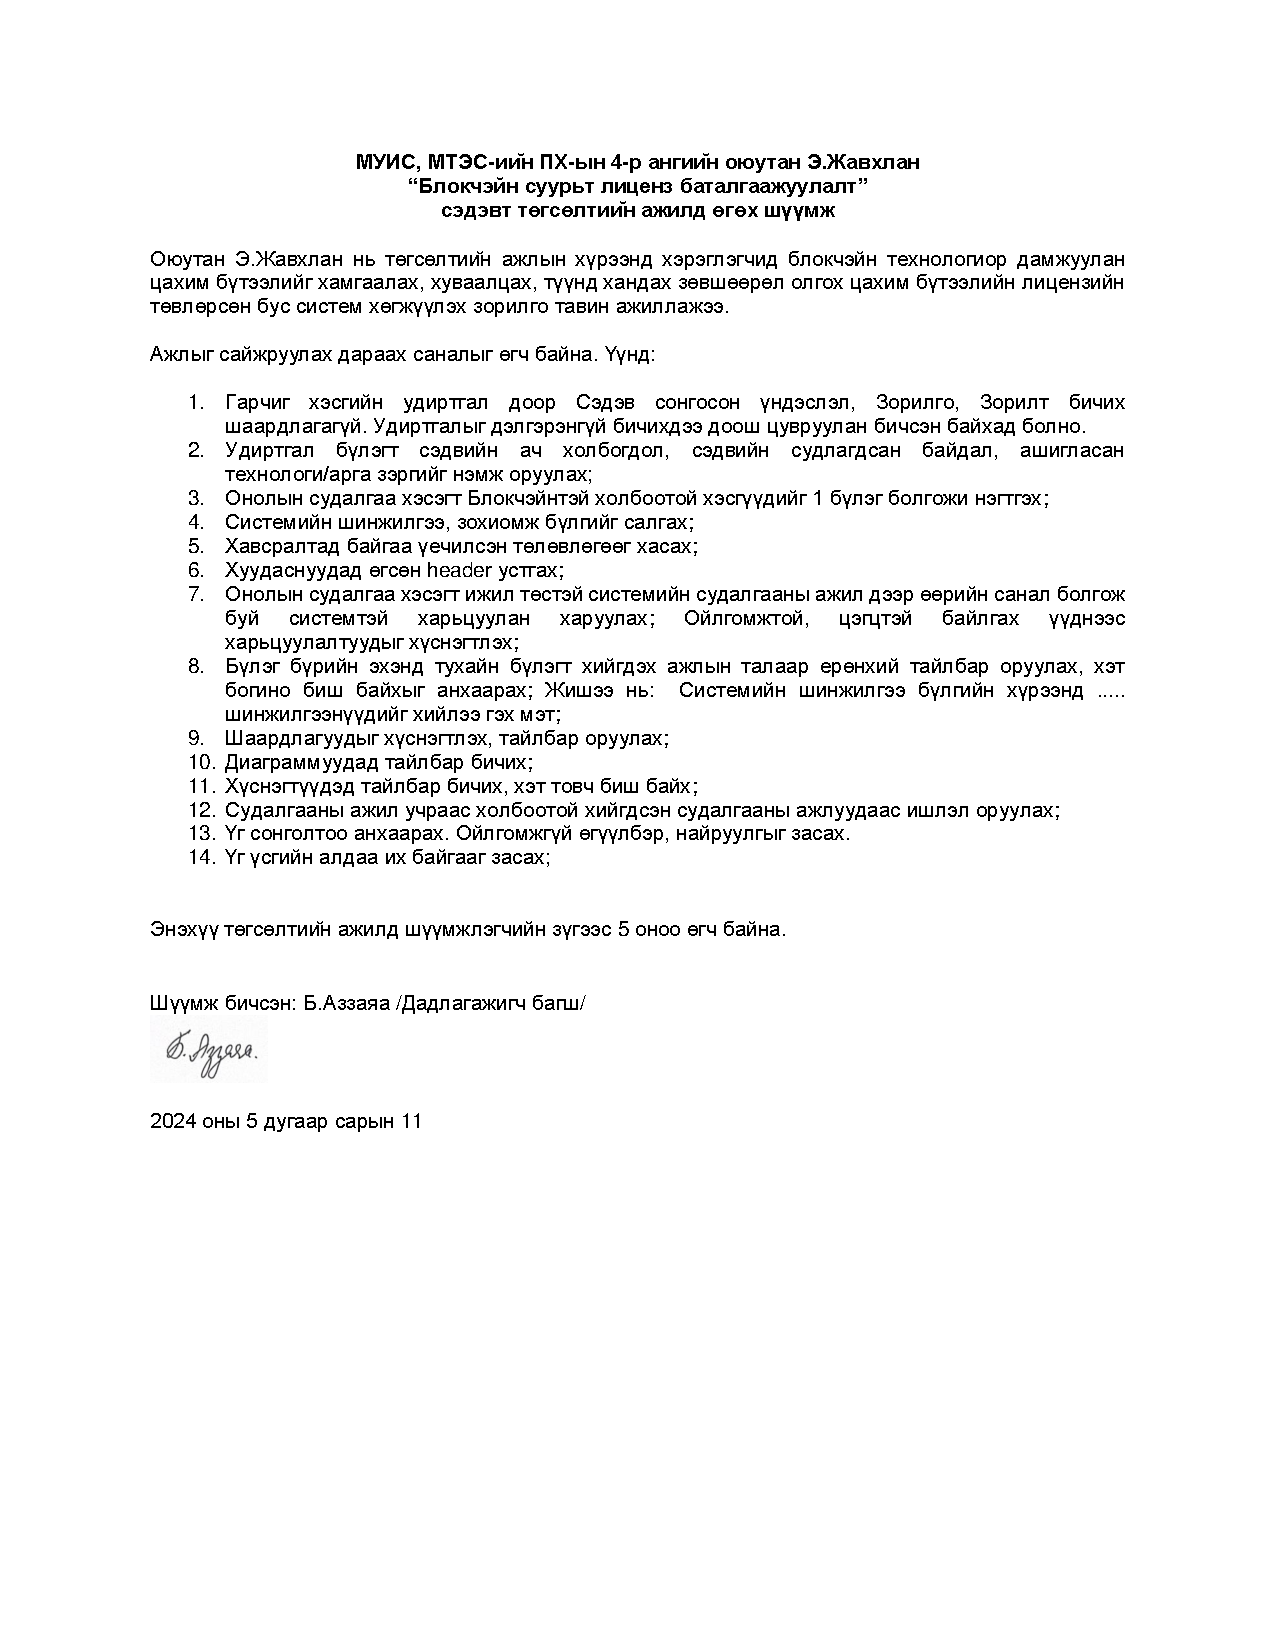
\includepdf[pages=1]{./src/review.pdf}
% Гарчгийг автоматаар оруулна
\setcounter{tocdepth}{1}
\tableofcontents

% Зургийн жагсаалтыг автоматаар оруулна
\listoffigures

% Хүснэгтийн жагсаалтыг автоматаар оруулна
\listoftables

% Кодын жагсаалтыг автоматаар оруулна
\lstlistoflistings

% This puts the word "Page" right justified above everything else.
\newpage
%% \addtocontents{lof}{Зураг~\hfill Хуудас \par}
\newpage
%% \addtocontents{lot}{Хүснэгт~\hfill Хуудас \par}

\renewcommand{\cftlabel}{Зураг}


\doublespace
\pagenumbering{arabic}


% Удиртгалыг оруулж ирэх ба abstract.tex файлд удиртгалаа бичнэ
\begin{abstract}
Миний бие \@author \ үйлдвэрийн дадлагын ажлыг “Зочил технологи” ХХК  компани дээр гүйцэтгэсэн. Энэхүү үйлдвэрийн дадлагын хүрээнд хичээлээс болон бие даан эзэмшсэн мэдлэг, чадвараа ашиглан бодит ажлын орчинд бүтээгдэхүүн хөгжүүлж бодит хэрэглэгчдийн гарт хүргэх процесст суралцан Админ веб удирдлагын систем төслийн front-end хөгжүүлэлтэнд оролцсон.

\textbf{Зорилго:} React, Bootstrap технологиудын талаар судалж бүтээгдэхүүн хөгжүүлэх, компанийн хөгжүүлэлтийн арга барилтай танилцах.

\textbf{Зорилт:} Удирдагчийн зааварчилгааны дагуу алхам алхмаар судалгаа хийж өгсөн шаардлагын хүрээнд хэрэгжүүлэлт хийх. Хурал уулзалтуудад хамрагдаж, бодит бүтээгдэхүүн хөгжүүлэлтийн процесст оролцох. Back-end хөгжүүлэлтийн багтай багаар хамтран ажиллах.

\end{abstract}


%----------------------------------------------------------------------------------------
%   Дипломын үндсэн хэсэг эндээс эхэлнэ
%----------------------------------------------------------------------------------------
%\addcontentsline{toc}{part}{БҮЛГҮҮД}
% Шинэ бүлэг
\chapter{Онолын судалгаа}
\subfile{src/chapters/chapter1.tex}
\chapter{Системийн шинжилгээ, зохиомж}
\subfile{src/chapters/chapter2.tex}
\chapter{Системийн хэрэгжүүлэлт}
\subfile{src/chapters/chapter3.tex}

%----------------------------------------------------------------------------------------
%   Дүгнэлт эндээс эхэлнэ
%----------------------------------------------------------------------------------------
% \chapter{Дүгнэлт}
Энэхүү судалгааны ажлаар блокчэйн технологи болон дижитал эрхийн менежментийн талаар судласан. Энэхүү судалж суралцсан мэдлэгээ ашиглан практикт цахим бүтээлийн лицензийн систем бүтээхийг зорилоо. Хөгжүүлэлтийн явцад блокчэйн сүлжээнд цахим бүтээлийг байршуулах, лиценз олгох, лицензийн баталгаажуулалт зэрэг янз бүрийн функцүүдыг хэрэгжүүлж, туршиж үзсэн.
\\
Үр дүнд нь орчин үеийн шинэлэг блокчэйн технологиудтай танилцсан ба бүтээгдэхүүний шаардлагыг гаргаж ухаалаг гэрээ бичихээс эхлээд эцсийн хэрэглэгчид хүрэх чанарын шаардлагыг хангаж блокчэйн технологийг ашиглан найдвартай, ил тод, төвлөрсөн бус системийг бүтээлээ.


%----------------------------------------------------------------------------------------
%   Дипломын номзүй, хавсралтын хэсэг эндээс эхэлнэ
%----------------------------------------------------------------------------------------

\singlespace
\addcontentsline{toc}{part}{НОМ ЗҮЙ}
\begin{thebibliography}{}
	% Ашигласан материалыг эндээс оруулна
   \bibitem{blockchain}
   Adam Hayes, Blockchain Facts: What Is It, How It Works, and How It Can Be Used. (December 15, 2023) \url{https://www.investopedia.com/terms/b/blockchain.asp}
   \bibitem{dlt}
   Scott Nevil, Distributed Ledger Technology (DLT): Definition and How It Works. (May 31, 2023) \url{https://www.investopedia.com/terms/d/distributed-ledger-technology-dlt.asp}
   \bibitem{zug_digtal_id}
    Sundararajan S. UN Agencies Turn to Blockchain In Fight Against Child Trafficking. (Nov 13, 2017)  \url{https://www.coindesk.com/markets/2017/11/13/un-agencies-turn-to-blockchain-in-fight-against-child-trafficking/}
   \bibitem{zug_digtal_id}
   Zug Digital ID: Blockchain Case Study for Government Issued Identity.  \url{https://www.investopedia.com/terms/b/blockchain.asp}
   \bibitem{drm}
   What is digital rights management (DRM)?.  \url{https://business.adobe.com/blog/basics/digital-rights-management}

\end{thebibliography}
\appendix
\addcontentsline{toc}{part}{ХАВСРАЛТ}

% Хавсралтын нэр. Хавсралт гэдэг үг агуулахгүй
\chapter{Үечилсэн төлөвлөгөө}
\begin{figure}[h!]
   \centering
   \includegraphics[scale=0.065, angle=90]{src/images/periodic-plan.png}
   \caption{Удирдагчийн үнэлгээ дүгнэлт}
\end{figure}


\chapter{Кодын хэрэгжүүлэлт}
\lstinputlisting[language=TypeScript, caption=Ухаалаг гэрээ,basicstyle=\linespread{0.6}\ttfamily,frame=single]{src/code/smart-contract.sol}

Уг код нь хэрэглэгчийн оруулах цахим бүтээлийг  мэдээллийг блокчэйнд бичнэ.
\lstinputlisting[language=TypeScript, caption=Блокчэйнд бичих,basicstyle=\linespread{0.8}\ttfamily,frame=single]{src/code/writeFile.ts}


Уг код нь хэрэглэгчийн оруулсан цахим бүтээлийн мэдээллийг блокчэйнээс уншина.
\lstinputlisting[language=TypeScript, caption=Блокчэйнээс унших,basicstyle=\linespread{0.8}\ttfamily,frame=single]{src/code/getUserFiles.ts}



%----------------------------------------------------------------------------------------
%   Хавсралтууд эндээс эхэлнэ
%----------------------------------------------------------------------------------------

\end{document}
